\documentclass[sigconf]{acmart}

\usepackage{booktabs} % For formal tables


% Copyright
%\setcopyright{none}
%\setcopyright{acmcopyright}
%\setcopyright{acmlicensed}
\setcopyright{rightsretained}
%\setcopyright{usgov}
%\setcopyright{usgovmixed}
%\setcopyright{cagov}
%\setcopyright{cagovmixed}


% DOI
\acmDOI{10.475/123_4}

% ISBN
\acmISBN{123-4567-24-567/08/06}

%Conference
\acmConference[FPGA'19]{ACM/SIGDA International Symposium on FieldProgrammable Gate Arrays}{February 24-26, 2019}{Seaside,California,USA}
\acmYear{2019}
\copyrightyear{2019}


\acmArticle{4}
\acmPrice{15.00}

\begin{document}
\title{Improving the Zynq-based DNN developer's ecosystem by integrating all necessary factors into a PYNQ-compliant online platform}
\titlenote{Produces the permission block, and
  copyright information}
%\subtitle{Extended Abstract}
%\subtitlenote{The full version of the author's guide is available as
 % \texttt{acmart.pdf} document}


\author{Chen Chen}
%\orcid{1234-5678-9012}
\affiliation{%
  \institution{School of IoT Engineering, Jiangnan University }
  \city{Wuxi}
  \country{China}
}
\email{6161910018@vip.jiangnan.edu.cn}

\author{Jun Xia}
\affiliation{%
  \institution{School of IoT Engineering, Jiangnan University }
  \city{Wuxi}
  \country{China}
}
\email{6161914036@vip.jiangnan.edu.cn}

\author{Wenmin Yang}
\affiliation{%
  \institution{OpenHEC Lab}
  \city{Wuxi}
  \country{China}}
\email{ouyang.wm@openhec.com}

\author{Kang Li}
\affiliation{%
  \institution{School of IoT Engineering, Jiangnan University}
  \city{Wuxi}
  \country{China}}
\email{6171966018@vip.jiangnan.edu.cn}

\author{Zhilei Chai}
\affiliation{%
  \institution{School of IoT Engineering, Jiangnan University \\Engineering Research Center of IoT Applications Ministry of Education }
  \city{Wuxi}
  \country{China}
}
\email{zlchai@jiangnan.edu.cn}


% The default list of authors is too long for headers.
\renewcommand{\shortauthors}{C. Chen et al.}


\begin{abstract}
The Zynq heterogeneous SoC from Xilinx is able to supporting software/hardware co-designing in one single chip, making it possible to take advantage of software flexibility and hardware acceleration at the same time. PYNQ project from Xilinx is trying to take advantage of high performance and low power consumption of Zynq while improve its programmability. In order to improve the ecosystem of PYNQ and help more embedded AI applications use the Zynq-based high-efficiency computational engine, this paper proposes a PYNQ-compliant online platform (OpenHEC-PYNQ) that integrates all necessary factors for the Zynq-based DNN developer. This platform makes HDL/HLS designers able to access all resources they needed via the Internet and finish all jobs one-stop. To show effectiveness of this platform, a YOLOv2 FPGA acceleration library is implmented based on OpenHEC-PYNQ. 
\end{abstract}

%
% The code below should be generated by the tool at
% http://dl.acm.org/ccs.cfm
% Please copy and paste the code instead of the example below.
%
\begin{CCSXML}
<ccs2012>
 <concept>
  <concept_id>10010520.10010553.10010562</concept_id>
  <concept_desc>Computer systems organization~Embedded systems</concept_desc>
  <concept_significance>500</concept_significance>
 </concept>
 <concept>
  <concept_id>10010520.10010575.10010755</concept_id>
  <concept_desc>Computer systems organization~Redundancy</concept_desc>
  <concept_significance>300</concept_significance>
 </concept>
 <concept>
  <concept_id>10010520.10010553.10010554</concept_id>
  <concept_desc>Computer systems organization~Robotics</concept_desc>
  <concept_significance>100</concept_significance>
 </concept>
 <concept>
  <concept_id>10003033.10003083.10003095</concept_id>
  <concept_desc>Networks~Network reliability</concept_desc>
  <concept_significance>100</concept_significance>
 </concept>
</ccs2012>
\end{CCSXML}

\ccsdesc[500]{Computer systems organization~Embedded systems}
\ccsdesc[300]{Computer systems organization~Redundancy}
\ccsdesc{Computer systems organization~Robotics}
\ccsdesc[100]{Networks~Network reliability}


\keywords{ACM proceedings, \LaTeX, text tagging}


\maketitle

\section{Introduction}
As its computational complexity, researchers and developers of the DNN (Deep Neural Network) were continuously seeking a suitable platform for implementation, in order to obtain high performance and low power consumption. The Zynq series heterogeneous SoC from Xilinx is able to supporting software/hardware co-designing in one single chip, making it possible to take advantage of software flexibility and hardware acceleration at the same time. Thus, increasing work of the DNN are developed on the Zynq recently. 

Those works of DNN's research based on Zynq mainly focus on four topics as follows. 
1) Micro-architecture designing for acceleration[7-18]. Different hardware structures were proposed such as Processing Elements, solicit arrays and pipeline to get higher performance with consideration of scalability. 
2) Memory bandwidth optimization[]. Such as reducing memory accessing frequency through storing intermediate result on chip[13,14], or enhancing the burst length by data reordering[7,11].
3) Matrix multiplication optimization[]. Such as Winograd, FFT transformation etc.
4) Model compression, pruning and quantization[]. those work concentrated on decreasing the complexity of computation.

However, although the heterogeneous SoC coupled with HLS(High Level Synthesis) improves description abstraction of system designing and frees users from non-trivial FPGA driver issues, it is more suitable for system-level programmers. It is because the programmer has to grasp knowledge of algorithm description, architecture and interfaces, physical address allocation, software drivers implementating and application software implementing. The drawback of this design flow is that system-level programmers generally have more architectural knowledge about hardware and software but fewer knowledge about algorithms and applications, and vise versa.

In order to expand the audience of zynq-based development ecosystem, Xilinx proposed PYNQ project, an open-source project that makes it easy to design embedded systems with Zynq SoCs. Using the Python language and libraries, designers can exploit the benefits of programmable logic and microprocessors in Zynq to build more capable and exciting embedded systems.

Neverthless, the success of PYNQ will rely on the abundance of libraries provided online, those are developed and submitted by the HDL/HLS designer. As for the DNN, HDL/HLS designers need to deal with non-trivial issues to develop and submit an FPGA-accelerated library, such as Neural Network model selection, quantization, re-tuning, hardware implementation, architectural designing, bitstream generation and software-hardware co-debugging etc. Many resources and tools are necessary to do all these work above such as datasets, deep learning framework, fixed-point quantitative tool, the Vivado toolkit, Zynq-based FPGA devices and boards. Generally, HDL/HLS designers need to learn and establish the developing environment including all these factors distributed everywhere by themselves from scratch, which is time-consuming and worthless. It prevents more contributors going into this field objectively.

Thus, this paper proposes a PYNQ-compliant online platform that integrates all necessary factors including Zynq devices for the Zynq-based DNN developer, so as to make it easier to contribute libraries under the PYNQ ecosystem. HDL/HLS designers will be able to access all resources they needed via the Internet and finish all jobs one-stop.

The main contribution of this paper is as follows:
\begin{enumerate}
    \item Establishing a PYNQ-compliant online platform. It brings all necessary datasets, tools, software and hardware resources together for the Zynq-based DNN developer, improving the PYNQ ecosystem.
    \item Taking YOLOv2, one of the current mainstream deep-learning algorithm, as an example to demonstrate the convenience of the online platform and contribute an open source project for PYNQ.
\end{enumerate}

\section{Factors involved in Zynq-based DNN development}
 When developing a DNN accelerator based on Zynq, the open source project, deep learning framework, datasets, fixed-point quantitative tool, the Vivado toolkit, Zynq-based FPGA devices and boards are all possibly used. This section introduces why all these factors should be put together for users convenience.

\subsection{Deep Learning Framework}
There are several mainstream frameworks such as Tensorflow, Caffe can be used. However, generally users need a plenty of time to establish the wanted framework on their own computers. 

\subsection{Datasets}
Besides training, when developing a Zynq-based DNN system, datasets are often necessary for weights tuning or re-tuning during the process of compression or pruning. The final optimized system also needs datasets to verify its correctness and accuracy. Generally, although some popular open datasets such as ImageNet or COCO can be found and downloaded from their official website, it is time-consuming for HDL/HLS designer instead of a deep learning researcher to find and get the suitable dataset distributed in different websites. Furthermore, it is even hard to get a suited dataset for emerging variant of the DNN model. 

For instance, the dataset of ImageNet has 13,000 training images (732 to 1,300 per class), 100,000 test images (100 per class) and 50,000 verified images (50 per class), its size is more than 100 Gigabytes.

\begin{figure*}
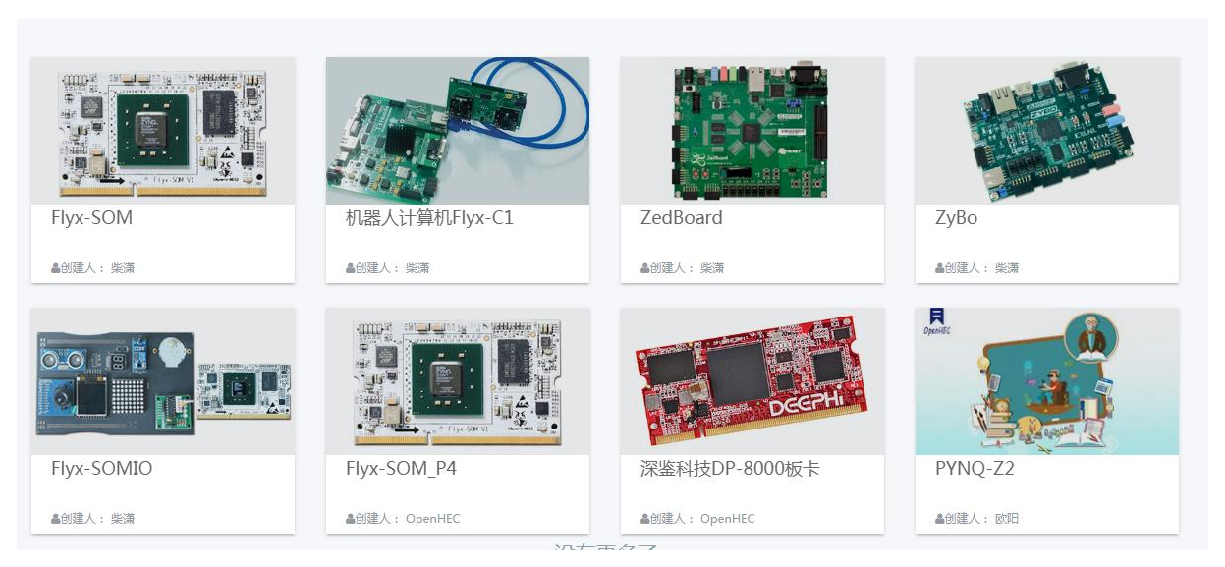
\includegraphics[height=3in, width=6in]{figure_1}
\caption{A sample black and white graphic.}
\end{figure*}

\subsection{Quantization tools}
One of the approache generally used for Zynq-based DNN optimization is bit-width compression of the datapath. Users can use one suitable tool to do datapath compression instead of doing it mannually. 
Presently, there are three kinds of quantization tools those are low-accuracy floating-point approximation, dynamic fixed-point approximation and weighting exponential fixed-point approximation. It is also a little difficult for HDL/HLS designers to find the suitable tool distributed everywhere.

\subsection{Vivado toolkit}
The Vivado toolkit for zynq-based devolopment including Vivado HLS, Vivado and SDK Xilinx is a neccessity for Zynq-based DNN developers. With continously increasing of the toolkit size, it is becoming harder to install and execute efficiently on individual user's own computer.

\subsection{Zynq-based FPGA devices and boards}
After simulation, synthesis and bitstream generation, FPGA devices or boards will be needed for verifying the running system with the Zynq-based DNN. In generall case, developers and researchers need to prepare their Zynq-based boards such as Zedboard etc. It is expensive to prepare and update the neccessary FPGA board with time and money.

As introduced above, Zynq-based DNN developers today still get facors needed for their research and development in a clumsy way. It impedes the Zynq-based high efficiency computing platform to be used in more embedded AI applications. 

\section{Pynq-compliant online plarform for DNN development}

\begin{figure}
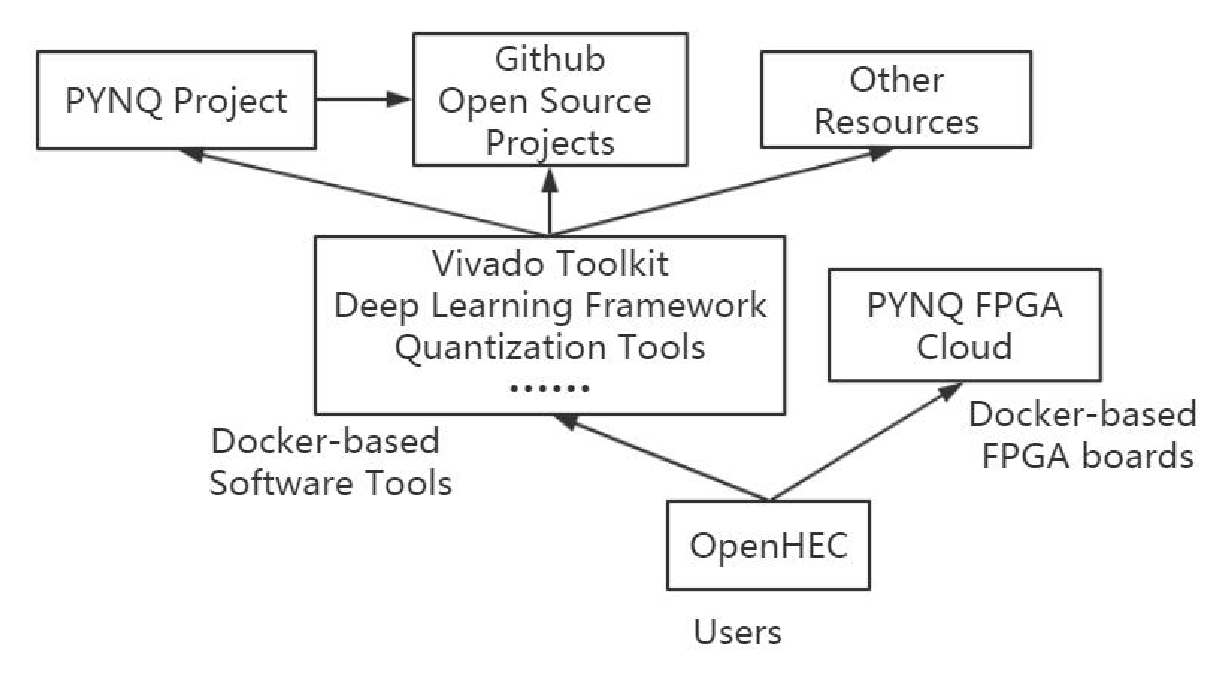
\includegraphics[height=1.7in, width=3.4in]{openhec}
\caption{Structure of OpenHEC-PYNQ platform}
\end{figure}

As shown in Fig.1, in this paper, a Pynq-compliant online plarform for DNN development, called OpenHEC-PYNQ for memorizing, was proposed to sovle the problem above. In this figure, OpenHEC is an FPGAs cloud platform at the website http://www.iopenhec.com, which provides remote accessing of the FPGA boards via the Internet. OpenHEC-PYNQ establishes the Pynq-compliant online plarform for DNN development through deploying Docker-based software tools such as Vivado toolkit and Docker-based PYNQ Z1/Z2 boards on the OpenHEC platform. As shown in this figure, users can use the Vivado toolkit, deep learning framework and quantization tool online during the Zynq-based DNN developing. Then, the bitsteam can also be downloaded and executed in PYNQ boards online conveniently via OpenHEC.
Other resources like open source projects at Github, datasets, PYNQ project and so on can be accessed via hyperlinks collected in OpenHEC. It avoids users to spend much time to find all the resources blindly.
At OpenHEC-PYNQ, the developer uploads the model to the cloud platform, and calls the framework and dataset online to train and test the network model. Developers can then use the tools provided by the platform to quantify the model and perform hardware design and optimization on the cropped network.

Figure xx shows the Docker-based software tools of OpenHEC-PYNQ, users can open and use the corresponding tool by double-click the icon.

Figure xx shows the entrance of OpenHEC-PYNQ for a specific PYNQ Z2 board. Once entering, the detailed information about the board can be viewed. The board can be accessed and used by just clicking the "using FPGA" button.

\begin{figure}
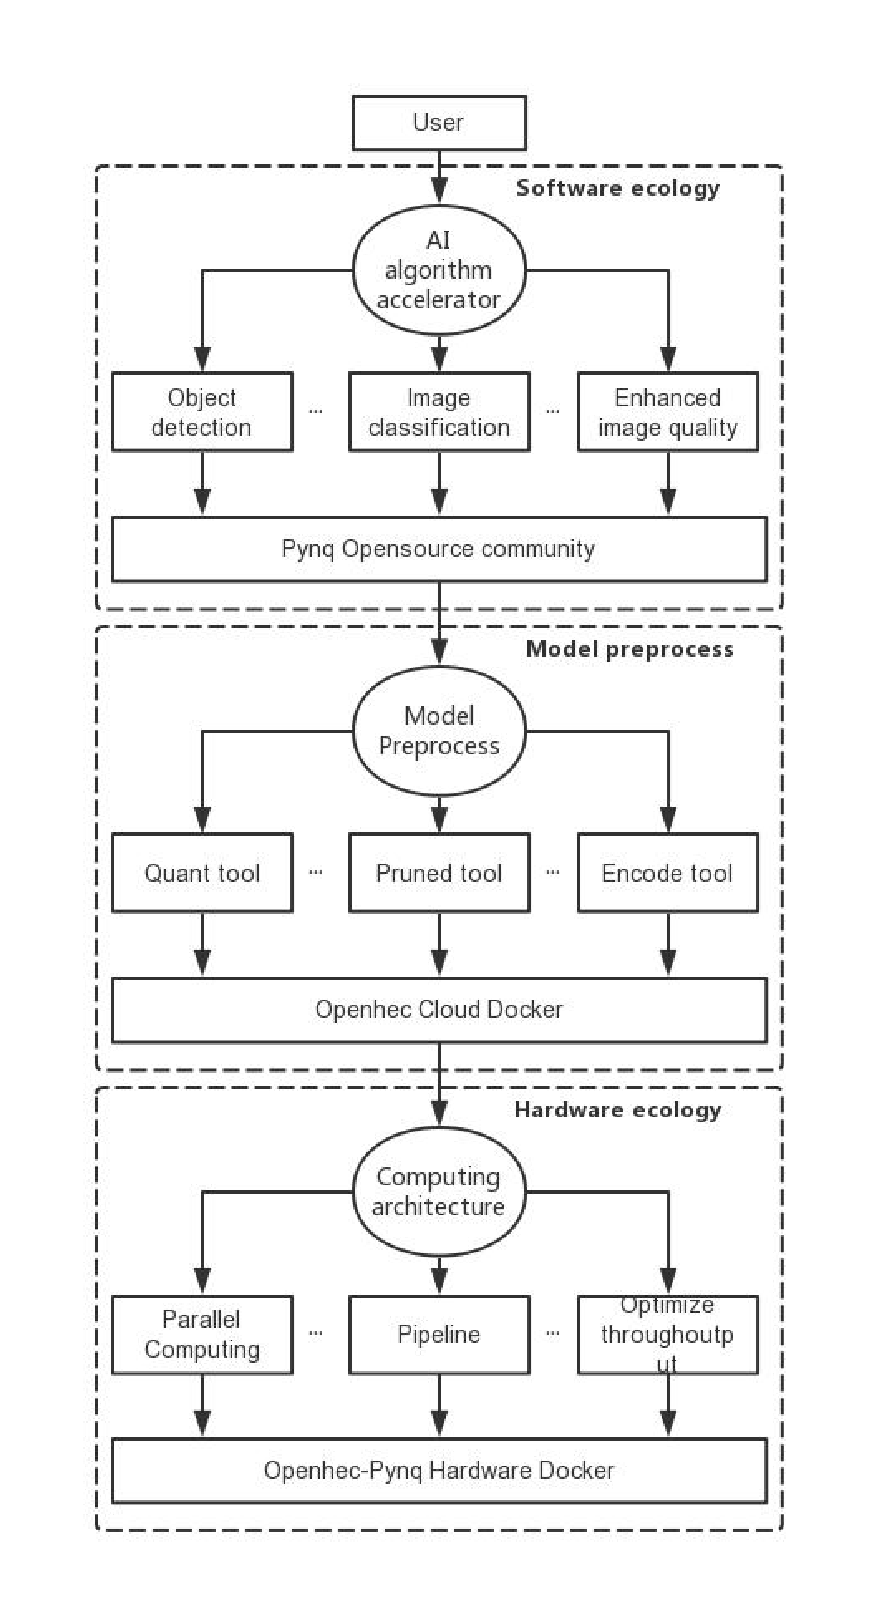
\includegraphics[height=7in, width=3.3in]{figure_0}
\caption{workflow}
\end{figure}

\section{Implementing YOLOv2 on Openhec-Pynq}
\subsection{About YOLOv2}
You only look once (YOLO) is a state-of-the-art, real-time object detection system. Using a novel, multi-scale training method the same YOLOv2 model can run at varying sizes, offering an easy tradeoff between speed and accuracy [21]. Currently, it has been recognized and invested in the field of ADAS [22, 23].

\subsection{Framework}
Darknet is an open source neural network framework written in C and provides the model of YOLOv2 [24]. We analyze the YOLOv2 network structure in Darknet, extract the required parameters and weights of each layer, and rewrite the C Model. Then, we verify the accuracy of the C model under float32 precision through the data set on the cloud platform.

\subsection{Quantization}
Since the Darknet framework itself does not have the quantization tool like Tensorflow or Pytorch. According to \cite{qiu2016going, shan2016dynamic}, we implement the precision conversion from float32 to fixed-16. Then, we verify the accuracy of the C model under fixed-16 precision.

\subsection{Optimizing YOLOv2 on Zynq FPGA}
According to the analysis of the YOLOv2 network, most layers are serially processed, except for the routing layer. The routing layer can be implemented by setting a specific address in advance. 

From an accelerator perspective, the work required is to interact with memory in order (reading memory data, processing data, and then writing back memory data). Since the amount of data input and output is very large, loop tiling technique is always applied to reuse data and reduce memory access times, which tiles the convolution loop R, C, M, N to Tr, Tc, Tm ,Tn\cite{zhang2015optimizing}.

The overall architecture of the accelerator is shown below:

\begin{figure}
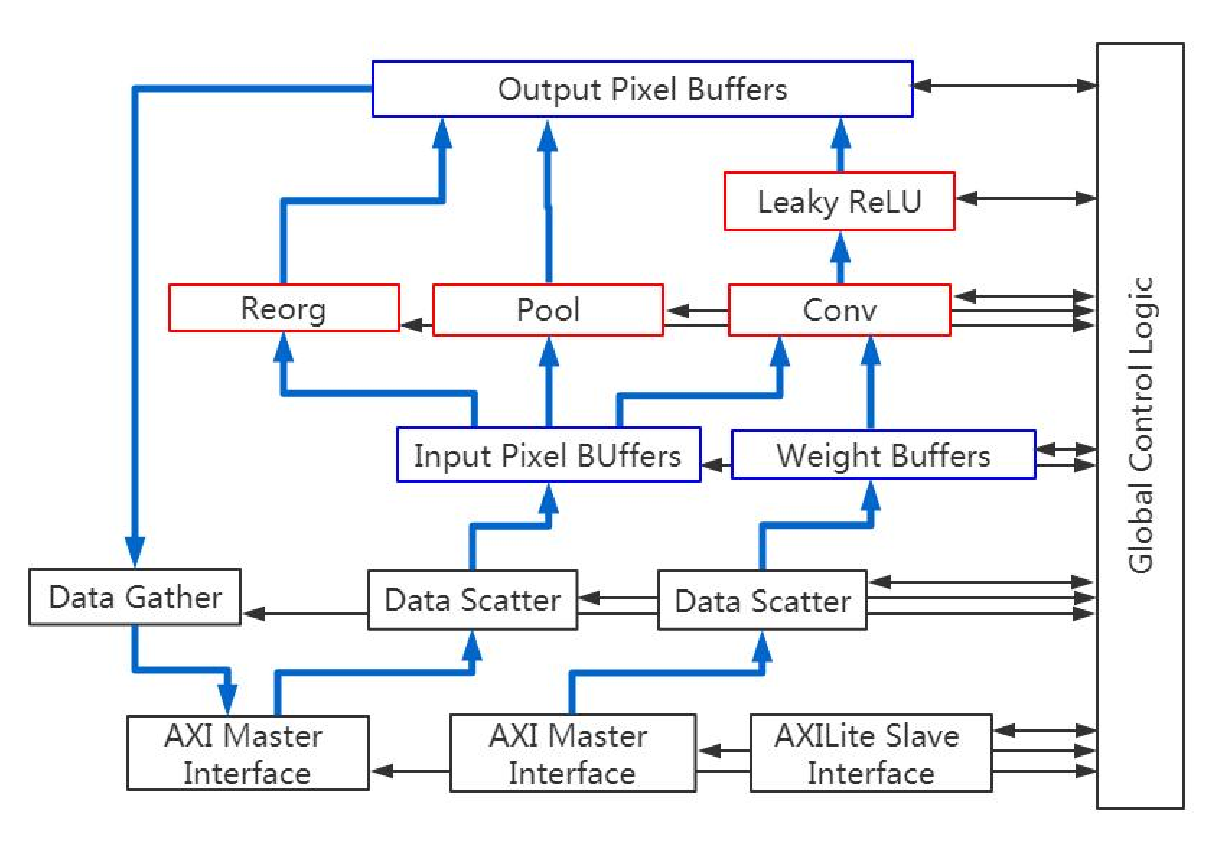
\includegraphics[scale=0.43]{figure_2}
\caption{XXX}
\end{figure}

Similar to \cite{zhang2015optimizing, chen2014diannao, ma2017automatic}, the accelerator has two AXI4 master interfaces and one AXI4-Lite slave interface. AXI-Lite slave interface is responsible for reading and writing control, data and status register sets. The input feature maps and weights are read concurrently by two master interfaces, and the output feature maps are written back simultaneously through write channel. 

The Data Scatter module is designed to generate the corresponding write address and distribute the data read from the DRAM to the on-chip buffers. The Data Gather module is designed to generate the DRAM write-back address and write the data in the output buffer back to the DRAM. The other red modules are responsible for the processing of the convolutional layer (Conv and Leaky ReLU), the maximum pooling layer (Pool) and the reorg layer (Reorg).

\begin{table*}
  \caption{Frequency of Special Characters}
  \label{tab:freq}
  \begin{tabular}{cccccc}
    \toprule
    {\quad}&DSP&BRAM&LUT&FF&Freq\\
    \midrule
    Fixed-16 & 106(48\%) & 100(72\%) & 27495(52\%) & 30118(28\%) & 130MHz\\
    Float-32 & 207(94\%) & 120(86\%) & 27816(52\%) & 27816(26\%) & 100MHz\\
  \bottomrule
\end{tabular}
\end{table*}

\begin{table*}
  \caption{Some Typical Commands}
  \label{tab:commands}
  \begin{tabular}{cccccc}
    \toprule
    {\quad}& \cite{ma2017hardware} & \cite{venieris2016fpgaconvnet}& \cite{wang2018pynq}&Ours&Ours\\
    \midrule
    CNN models & Tiny-YOLO v1& Scene Labelling&LeNet-5&YOLO v2&YOLO v2 \\
    FPGA Board(FPGA) & VC707(Virtex7 485t) & Zedboard(XC7Z020) & Pynq(XC7Z020) & Pynq(XC7Z020)& Pynq(XC7Z020)\\
    Clock(MHz) & 143 & 100 & 100 & 100 & 130\\
    Precision & Fixed-16 & Fixed-16 & Fixed-8 & Float-32 & Fixed-16\\
    Power(W) & - & 1.75 & 1.90 & 2.39 & 2.71\\
    Operations(GOP) & 3.09 & - & $4.58*10^{-3}$ & 29.47 & 29.47\\
    Performance(GOP/s) & 64.86 & 12.73 & 2.56 & 2.53 & 11.39\\
    Power Efficiency(GOP/s/W) & - & 7.27 & 1.35 & 1.06 & 4.20\\
    \bottomrule
  \end{tabular}
\end{table*}

\subsubsection{Weight Arrangement}
The effective FPGA bandwidth goes up with the increase of burst length and finally flattens out above some burst length threshold\cite{zhang2016caffeine}. The data tiling technique usually results in a discontinuous DRAM access for the row-major data layout in DRAM. To reduce the number of memory accesses and increase the effective memory bandwidth, we arrange the kernel weights for an entire tile to a continuous block to ensure a high utilization of the bandwidth of external memory \cite{qiu2016going}.

\subsubsection{Parallel Convolution Engine}
The acceleration strategy of convolutional layer is similar to \cite{zhang2015optimizing, motamedi2017placid}, which utilizes input and output parallelism to accelerate the computation. By designing multiple parallel multiplication units and add trees to achieve input parallelism (Tn parallelism) and output parallelism (Tm parallelism) in convolution calculation. The Tm*Tn multiplication units are calculated in parallel. The add trees of Log2 (Tn) depth are accumulated by pipeline, and generate the partial sums.

\subsubsection{Ping-Pong operation}
Similar to \cite{zhang2015optimizing}, the design implements ping-pong buffers to overlap the delay of reading input feature maps and weights, writing output feature maps and calculation, which greatly improves the dynamic utilization of the computing engines.

\subsection{Python interface}
After completing the accelerator design, we used Python to write the driver for the accelerator. Verify the accuracy of the actual designed accelerator through the Python interface.

\section{Results and Comparison}
Two data precision types of float32 and dynamic fixed-point 16-bit have been designed. Experiments show that floating point addition in HLS requires three DSP resources, floating point multiplication requires two DSPs; fixed point 16-bit multiplication requires one DSP, and fixed-point 16-bit addition can be implemented only using LUT. After placing and routing, resource consumptions of float32 (Tn=3, Tm=9, Tr=26, Tc=52) and fixed-16 (Tn=2, Tm=32, Tr=26, Tc=26) are shown as table 1.

According to the current design, DSP and BRAM are more expensive. The cost of DSP can be further reduced (there are many bit-width redundant multiplications), and the BRAM cost can be reduced. (As Shen \cite{shen2017maximizing} said, BRAM allocates an exponential size of 2 in HLS. Actually, many BRAMs are redundant.).

The performance comparison in the two cases is shown in table2.

\cite{wang2018pynq} is also based on the PYNQ ecosystem, but the demo given is a simple LeNet-5 and is based on a full-pipeline architecture. Most of the current networks are more complex and larger than LeNet-5. Considering the cost and power consumption of embedded FPGAs, the examples are not well presented, and they are less than us in performance and energy efficiency. 

In \cite{venieris2016fpgaconvnet}, the dynamic reconfiguration is used to process 254 images in batches for reducing the reconstruction cost, which makes the performance and energy efficiency very high. However, in practical applications, there are few occasions where such large quantities are required, and tend to low latency.

\cite{ma2017hardware} implemented tiny-yolov1 on a middle-range FPGA. The tiny-yolov1 model is relatively backward, and the FPGA used has a large power consumption, which is not suitable for embedded applications.

\section{Conclusions}
PYNQ project from Xilinx is trying to partition developers on Zynq SoCs into two categories: Software developers using Python through calling libraries of hardware acceleration to get high performance and low power consumption. Hardware developers who use HDL/HLS to design and contribute libraries of hardware acceleration. The success of this ecosystem denpends on the abundance of libraries provided. This paper proposed a Pynq-compliant online plarform for DNN development to make the HDL/HLS designer to contribute libraries of hardware acceleration much easier. It will potentially improve the ecosystem of PYNQ and help more embedded AI applications use the Zynq-based high-efficiency computational engine.

\begin{acks}
  The authors would like to thank Dr. Yuhua Li for providing the
  MATLAB code of the \textit{BEPS} method.

  The authors would also like to thank the anonymous referees for
  their valuable comments and helpful suggestions. The work is
  supported by the \grantsponsor{GS501100001809}{National Natural
    Science Foundation of
    China}{http://dx.doi.org/10.13039/501100001809} under Grant
  No.:~\grantnum{GS501100001809}{61273304}
  and~\grantnum[http://www.nnsf.cn/youngscientists]{GS501100001809}{Young
    Scientists' Support Program}.

\end{acks}


\bibliographystyle{ACM-Reference-Format}
\bibliography{bib_20180926_1602}

\end{document}
